\documentclass[tikz,border=2mm]{standalone}
\usepackage{tikz}
\usetikzlibrary{arrows,positioning}
\usepackage{pgfplots}
\usepackage{amsmath,mathtools}
\usepgfplotslibrary{fillbetween}
\pgfplotsset{compat=1.17}
\begin{document}
% Picture 1: simulated data ZOOMED IN 
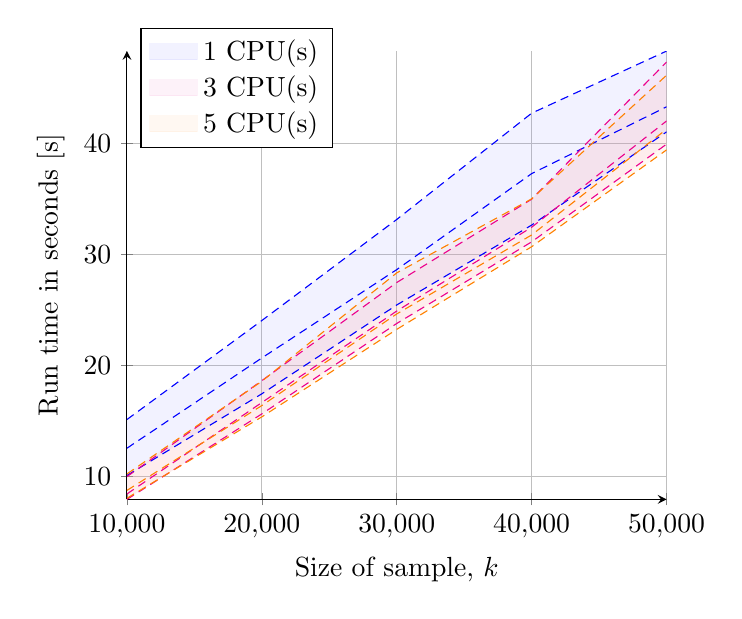
\begin{tikzpicture}
\begin{axis}[
    axis lines=left, %xtick=\empty, ytick=\empty.
    grid=both,
    ylabel style = {align=center},
    scaled x ticks = false,
    xlabel = {Size of sample, $k$},
    ylabel = {Run time in seconds $[\mathrm{s}]$},
    legend style={at={(axis cs:11000,45)},anchor=west,cells={align=center},nodes={scale=1.0}},
]
% Include the simulated data
\addplot[forget plot,densely dashed,color=blue,name path=down]coordinates {
	(10000.0000	,	10.0696)
	(20000.0000	,	17.4237)
	(30000.0000	,	25.4273)
	(40000.0000	,	32.6244)
	(50000.0000	,	41.0251)
};
\addplot[forget plot,densely dashed,color=blue]coordinates {
	(10000.0000	,	12.5235)
	(20000.0000	,	20.6558)
	(30000.0000	,	28.6139)
	(40000.0000	,	37.2617)
	(50000.0000	,	43.2793)
};
\addplot[forget plot,densely dashed,color=blue,name path=up]coordinates {
	(10000.0000	,	15.1075)
	(20000.0000	,	24.0257)
	(30000.0000	,	33.1333)
	(40000.0000	,	42.7053)
	(50000.0000	,	48.3017)
};
\addplot[blue!50,opacity=0.1] fill between[of=up and down];
\addlegendentry{1 CPU(s)}
\addplot[forget plot,densely dashed,color=magenta,name path=down]coordinates {
	(10000.0000	,	7.9133)
	(20000.0000	,	15.6142)
	(30000.0000	,	23.7607)
	(40000.0000	,	31.1134)
	(50000.0000	,	39.9163)
};
\addplot[forget plot,densely dashed,color=magenta]coordinates {
	(10000.0000	,	8.4008)
	(20000.0000	,	16.6397)
	(30000.0000	,	24.8816)
	(40000.0000	,	32.4314)
	(50000.0000	,	42.0057)
};
\addplot[forget plot,densely dashed,color=magenta,name path=up]coordinates {
	(10000.0000	,	9.9627)
	(20000.0000	,	18.6096)
	(30000.0000	,	27.4517)
	(40000.0000	,	34.9565)
	(50000.0000	,	47.3116)
};
\addplot[magenta!50,opacity=0.1] fill between[of=up and down];
\addlegendentry{3 CPU(s)}
\addplot[forget plot,densely dashed,color=orange,name path=down]coordinates {
	(10000.0000	,	8.0167)
	(20000.0000	,	15.3485)
	(30000.0000	,	23.2296)
	(40000.0000	,	30.6760)
	(50000.0000	,	39.3977)
};
\addplot[forget plot,densely dashed,color=orange]coordinates {
	(10000.0000	,	8.7229)
	(20000.0000	,	16.3694)
	(30000.0000	,	24.6208)
	(40000.0000	,	31.7365)
	(50000.0000	,	41.2653)
};
\addplot[forget plot,densely dashed,color=orange,name path=up]coordinates {
	(10000.0000	,	10.2035)
	(20000.0000	,	18.5593)
	(30000.0000	,	28.3208)
	(40000.0000	,	34.9886)
	(50000.0000	,	46.1267)
};
\addplot[orange!50,opacity=0.1] fill between[of=up and down];
\addlegendentry{5 CPU(s)}
\end{axis}
\end{tikzpicture}



\end{document}
